\chapter{Implementation}
\label{chap:03_implementation}

\missing[inline]{
    * Alsa\\
    * Where in HULKs code and general HULKs framework\\
    * How WhistleLocalization is introduced into framework\\
    * Show that channel signals from front and rear have same mean magnitude\\
    * TDOA\\
    \tab * CC Implementation\\
    \tab * GCC Implementation\\
    \tab * Phase Diff Implementation\\
    * Rear distance calculation\\
    * How TeamWhistleLocalization is implemented\\
    * Also mention things that did not work:\\
        \tab * SNR\\
        \tab * Magnitude to check rough direction
}

% phase method: assumes that the signal comes from
% the direction with higher amplitude
% only 3 pairs are used

\section{Nao Framework}
\label{sec:03_whistleLocalizationModule}

The direction of a whistle sound source is calculated after a whistle sound was detected
by the existing \lstinline!WhistleDetection! module.

\subsection{Coordinate System}
\label{subsec:03_coordinates}

Next channel is always defined as the right adjacent channel.

\subsection{Existing Whistle Detection}
\label{subsec:03_whistleDetection}
\subsection{Signal Start Detection}
\label{subsec:03_signalStartDetection}

As mentioned in \cref{sec:02_signalStartDetection}, the detection of the
signal start is crucial for the localization.
The implementation of the different approaches will be presented coupled with
an examination of real measurement data.
To reduce undesirable effects and demonstrate the simplest form, a sinusoidal
signal of $3\si{\kilo\hertz}$ was recorded with the same circumstances as the
whistle sounds.
For the following data, the sound source was placed $2\si{m}$ in front of the robot.
In order to find the time point where the signal starts, information about
smaller fractions are required.
So, the original $44100$ samples that were buffered by the
\lstinline!WhistleLocalization! module are divided into several overlapping
frames with size $256$. The computational effort raises with smaller frame size,
but delivers a higher precision in return.
In order to perform the \ac{FFT} most efficiently, the size of one frame
should be a power of 2.
To compute the energy and entropy, the frames are transformed into
frequency domain with the \ac{FFT}.
The \ac{ZCR} does not require such a transformation.
In the evaluation \cref{sec:04_signalStartDetection}, the result of the single
methods are compared to each other.
For better visualization, the following data is shortened to $2400$ samples.

\missing[]{Start detection by frequency, whistle detection}

\subsubsection*{Spectral Entropy}

The formula to calculate the spectral entropy of a signal is introduced as
\cref{eq:02_entropy} in the previous chapter.
For the entropy information, the signal must not be cleaned previously.
By looking at the derivation of the entropy, a global minimum can be found
at the starting point of the signal due to its change from noise to signal.
The starting index is therefore defined by the index of the derivation's minimum.
Of course, this approach does not work real-time but with small delay.
\Cref{fig:03_entropy} is a plot of the recorded sine signal with the corresponding
entropy.
According to the frame size, the accuracy of the start index can be increased.
However, the frame size is limited by the required number of samples for one \ac{FFT} and
its computational effort.
% -------------------------------------------------------------
\begin{figure}[ht]
	\centering
		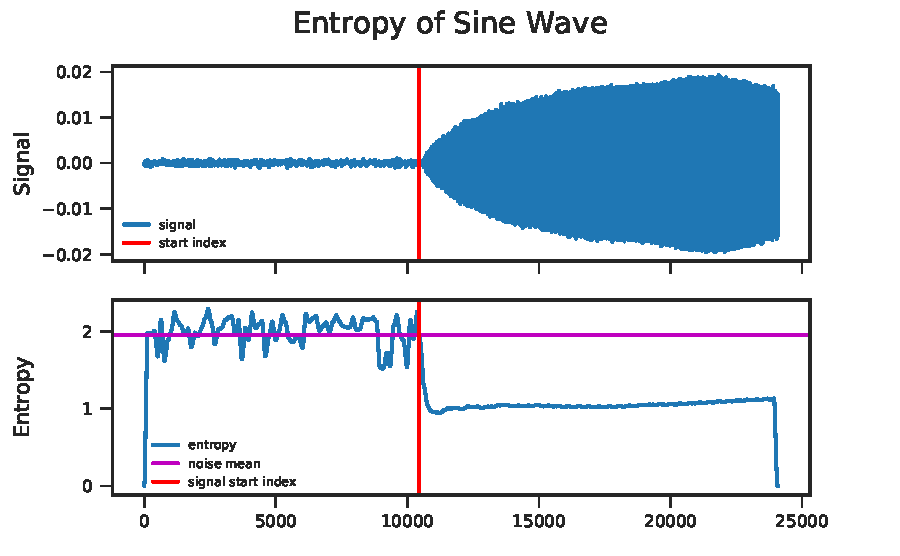
\includegraphics[]{figures/sine_entropy}
	\caption{Exemplary entropy of a sinusoidal signal with 3\si{\kilo\hertz}.}
	\label{fig:03_entropy}
\end{figure}
% -------------------------------------------------------------
In \cref{subsec:04_entropy}, the entropy outcome of a whistle sound
and its derivation is presented for evaluation.

\subsubsection*{Energy}

As mentioned above, the total signal is divided into multiple overlapping frames.
\Cref{eq:02_spectralEnergy} represents the energy of each frequency
component.
According to this, the energy of one of those frames is \cref{eq:02_energy}.
Assuming that the energy holds for the whole frame, overlapping and adding the energy
results in \cref{fig:03_energy}.
If the frequency of the examined signal is known as for the whistle, only energy values
of the relevant frequencies needs to be considered.
One downside of the energy information is that the threshold has to be adapted
manually for the related environment.
Especially at the tournament, parameters like these should be avoided and thus,
the start detection by energy is inconvenient.
% -------------------------------------------------------------
\begin{figure}[ht]
	\centering
		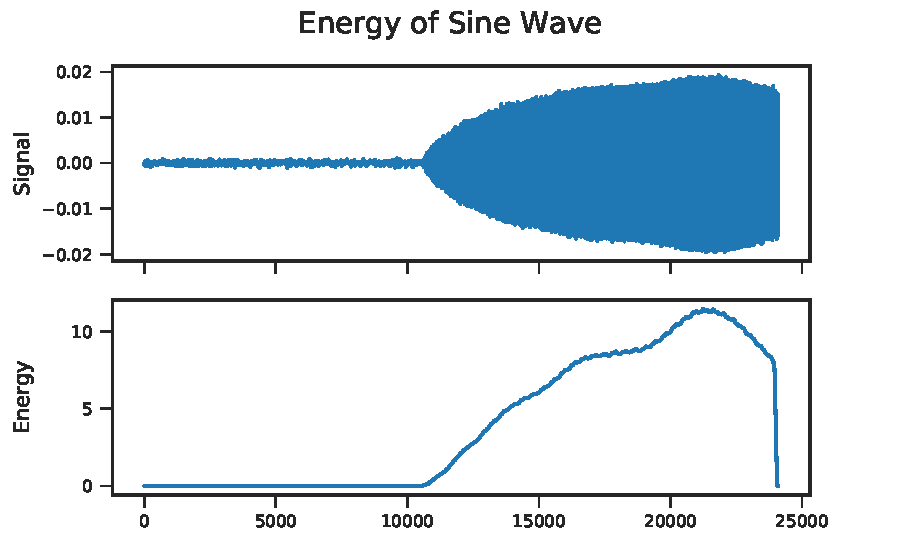
\includegraphics[]{figures/sine_energy}
	\caption{Energy of a sinusoidal signal with 3\si{\kilo\hertz}.}
	\label{fig:03_energy}
\end{figure}
% -------------------------------------------------------------

\subsubsection*{Zero Crossing Rate}

Alike the other methods, the buffered signal is divided into smaller frames
which can be set arbirary small for the \ac{ZCR} where no \ac{FFT} is necessary.
% To receive a higher accuracy, the frames of the \ac{ZCR} can be set small.
% are set to 80 samples.
In each frame, the sign changes are counted which only requires simple implementation
and computationally lightweight.
It is known that only noise is received at the beginning of the measurement and on the
contrary, signal noise is present at the end.
By comparing the mean of the received noise at the beginning of the measurement and
the mean of the signal part, a dynamic threshold can be defined and the beginning of the
signal is detectable.
In this work, the crossing of the threshold is observed from the last
value to the first.
Number of noise and signal frames are parameter values which depend
on the amount of samples and the size of the frame.
% In \cref{fig:03_zcr} and in this work, the threshold is set by multiplying the
% mean of the noise and signal mean by factor 1,25.
\begin{figure}[ht]
	\centering
		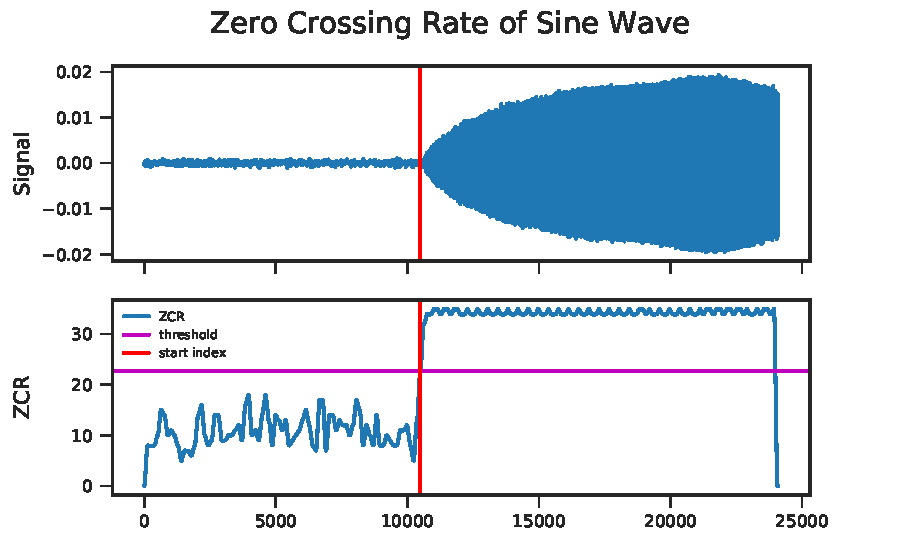
\includegraphics[]{figures/sine_zcr}
	\caption{Zero Crossing Rate of a sinusoidal signal with 3\si{\kilo\hertz}.}
	\label{fig:03_zcr}
\end{figure}
According to the circumstances, the threshold can be lowered optionally.
For real whistle data, the mean of noise and signal mean is reduced by factor 0,9 to
lower the threshold and results are shown in \cref{subsec:04_zcr}.

\section{Delay Estimation}
\label{sec:03_delay}

To ascertain the direction of the sound source on one robot, the
delay of the signal from each channel to it's neighboring
next channel is the key information.
The implementation of the \ac{CC} from \cref{sec:02_cc} and the \ac{GCC-PHAT}
introduced in \cref{sec:02_gcc}, as well as the phase difference method
of \cref{sec:02_phase} will be presented shortly.

For all methods performed in frequency domain, the \ac{FFT} of the
signal is required. Hence the library NumPy for Python codes, known for it's high-level
mathematical functions also provides a module with fundamental
functions for the \ac{DFT}, \lstinline!numpy.fft.fft()! and
\lstinline!numpy.fft.ifft()! can be utilized.
In C++, the library \ac{FFTW} exists and delivers the same \ac{DFT} functions.
To estimate the delay between \lstinline!signal_0! and \lstinline!signal_1!,
both frames of the signals were Hann windowed in advance.
% -------------------------------------------------------------
\subsection*{Correlation}
\label{subsec:03_cc}

In Python, using the \ac{DFT} functions given by NumPy the \ac{CC} and \ac{GCC} calculation
can be implemented with little lines of code.
% Function \lstinline!correlation! of \cref{lst:03_cc} itemizes the steps to accomplish
\missing[]{text}
a correlation in Python with input signals \lstinline!x0! and \lstinline!x1!.
Determining the index of the maximal value of the correlation relative to the zero delay
index delivers the delay of \lstinline!x1! compared to \lstinline!x1! as the function
\lstinline!compute_delay! demonstrates.
% -------------------------------------------------------------
\subsection*{Subsample Delay}
\label{subsec:03_subsample}

Integer delays only offers resulting direction angles with low resolution.
To avoid this, the subsample shift estimation as in \cref{sec:02_subsampleShift}
is added to the delay estimation.

\subsection*{Phase Difference}
\label{subsec:03_phase}

There are two ways to determine the angle by phase difference
between two channels.
One can either look at the phase of a fixed frequency or set the frequency
dynamically.
For both, the signal must be divided into multiple frames.
The implementation for the fixed frequency case is straight forward.
From the result of the signal start detection, the frames
are set with an appropriate frame size and then transformed into
frequency domain.
As we know, the frequency of the whistle is between 2\si{\kilo\hertz}
and 4\si{\kilo\hertz}.
Thus, a suitable frequency in this range is chosen for analysis.
In the other case, the frame is chosen by doing a
frequency analysis.
For each channel frame in frequency domain after signal start,
the maximal absolute value and its belonging frequency is determined.
If this frequency is equal for all channels, these frames
are chosen.
\Cref{fig:03_maxFreq} shows that such frames exists for signals that
were transformed into frequency domain with a frame size of 256.
The frequency resolution changes with zero padding the signal prior
to the transformation.
\change[]{Finalize!}
% -------------------------------------------------------------
\begin{figure}[ht]
	\centering
		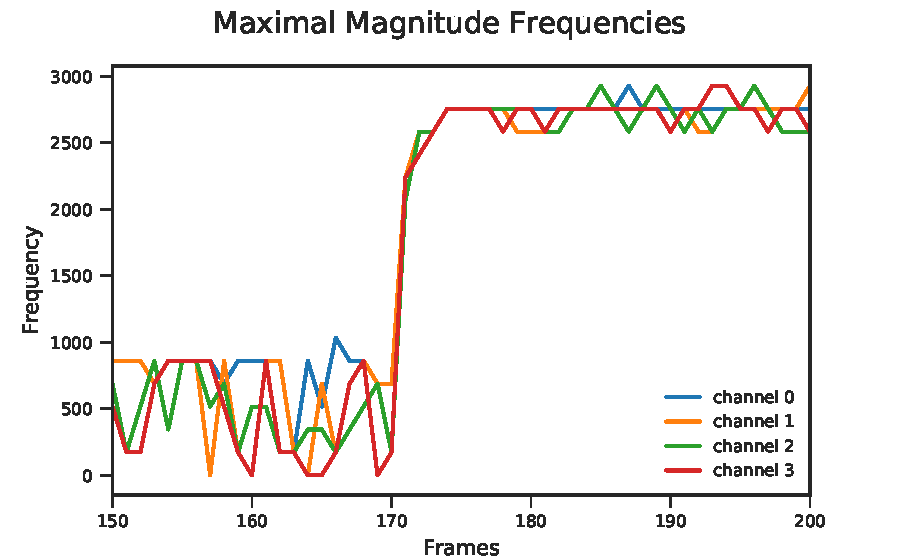
\includegraphics[]{figures/maxFreq}
	\caption{}
    \label{fig:03_maxFreq}
\end{figure}
% -------------------------------------------------------------

If the \ac{TDOA} is determined by phase difference, it must be ensured
that the maximal difference between two channels must not overflow $\pi$.
Meeting this condition, the signed difference is ascertainable.
As \cref{tab:03_maxFrequncies} presents, the distance between channel 0 and 1
is too large because its maximal frequency is not in whistle frequency range.
For this reason, the phase difference information between this pair is neglected.
% -------------------------------------------------------------
\btline{ht}{1.2}
\btab{|c|c|c|}
\hline
Channel Pairs & Absolute Distance [\si{\meter}] & Frequency [\si{\hertz}]\\
\hline
0 and 1 & 0,116 & 1536,75\\
\hline
1 and 3 & 0,0533 & 3217,11\\
\hline
2 and 0 & 0,0533 & 3217,11\\
\hline
2 and 3 & 0.0618 & 2775,08\\
\hline
\etab
\et{Maximal feasible frequencies for unambiguous phase difference detection}{03_maxFrequncies}
% -------------------------------------------------------------

To facilitate the implementation, the phase difference is easily convertible into
delay samples $D_s$ with
\bal
	D_s = \frac{f_s \cdot \Delta \psi}{2 \pi \cdot f_c}.
\eal
\section{Front and Rear Distance}
\label{sec:03_distance}

If the front and rear direction candidates dissolve each other to a small
value, it is assumed that the signal source is on the X-axis of the robot.
The side delays are then used as indicator for the distance to the robot as
explained in \cref{sec:02_distance} and need to be smaller than
\change[]{change name?} $samples_{xz}$.
To estimate the distance, the height of the sound source needs to be set as
constant \change[]{change name?} \lstinline!height_source!.\\
Restrictions of the front and rear distance measurement differ.
For the front case, the maximal angle for a unambiguous distance calculation
is $\frac{\pi}{2}- 2\alpha$.
Thus, the maximal front distance that can be approximated shrinks to
$\Delta x = (\Delta h_{source} - \Delta h_{Nao}) \cdot \tan(\frac{\pi}{2} - 2\alpha)$
according to \cref{eq:02_deltaX}.
To the rear, the maximal value for $\gamma$ is bounded by \change[]{naming?}
\lstinline!xz_delay_limit!.
Setting $\Delta h_{source}$ to 1.5\si{m} and $\Delta h_{Nao}$ to 0.57\si{m},
the maximal measurable distance to the front is about 0.66\si{m}.
With the same values and 5.3 samples as \lstinline!xz_delay_limit!, the
minimum $\Delta x$ value is 33.29\si{m}.
\code{distance}{0}{35}{Pseudo code of distance approximation on X-axis.}{03_distance}
\unsure[]{I am not really sure how pseudo codes should look like and if one is necessary anyway?}

\section{Direction Estimation}
\label{sec:03_direction}

After the \lstinline!WhistleData! was filled by the \lstinline!WhistleDetection!,
the \lstinline!WhistleLocalization! start to process the buffered microphone data.
First, the frames which will be considered for the calculation of the \ac{TDOA}
are chosen.
Different criteria apply for the correlation methods and phase method, but the
resulting \lstinline!start_index! of the signal start detection implementation
\cref{sec:03_signalStartDetection} is utilized in both.
% -------------------------------------------------------------

For the correlation methods in \cref{sec:02_cc} and \cref{sec:02_gcc}, the beginning
of the signal is chosen where the change from noise to signal is visible at best.
\lstinline!frame_size/2! samples before and after the \lstinline!start_index! are defined
as frame.
It gets undecidable which signal came first for later frames. Thus, if the start detection
is inaccurate the resulting \ac{TDOA} is not reliable.
% -------------------------------------------------------------

Regarding the phase method,
%\cref{sec:02_phase}%,
\missing[]{reference to 02 phase}
the frames with the same maximal frequency for each channel are used for the
phase difference calculation.
The phase difference of this frequency is then considered for the phase difference
calculation. %\cref{sec:03_phase}
\missing[]{reference to 03 phase}
% -------------------------------------------------------------

Before determining the delays, the frames are windowed with a Hann window and can be
normalized optionally.
According to the method, the delays between the channels are computed to conclude the
consequential direction candidates.
For each delay between neighboring channels, one positive signed and one negative
signed candidate arise.

% -------------------------------------------------------------
\Cref{lst:03_direction} lists the single steps that are necessary for the sound source
candidates in robot coordinates.
Positive values for delays mean that the signal first arrived at the \lstinline!base_channel!.
Exemplary considering the case where the delay is equal to the positive maximal delay,
the signal was first
detected by the \lstinline!base_channel! before arriving at the \lstinline!next_channel!.
As a consequence, the direction of the source is opposite to the channel vector and equal
to the \lstinline!max_delay_vector!.
Generally, the direction candidates are calculated relative to this \lstinline!max_delay_vector!,
where the angle $\gamma'$ is determined by \cref{eq:02_tdoaAngle}.
\Cref{fig:03_tdoaCode} shows resulting candidates of same situation as \cref{fig:02_tdoa} with
the resulting possible source directions \lstinline!candidates!.
% -------------------------------------------------------------
\code{tdoa}{0}{10}{Calculation of whistle direction in robot coordinates.}{03_direction}
% -------------------------------------------------------------
\begin{figure}[ht]
	\centering
		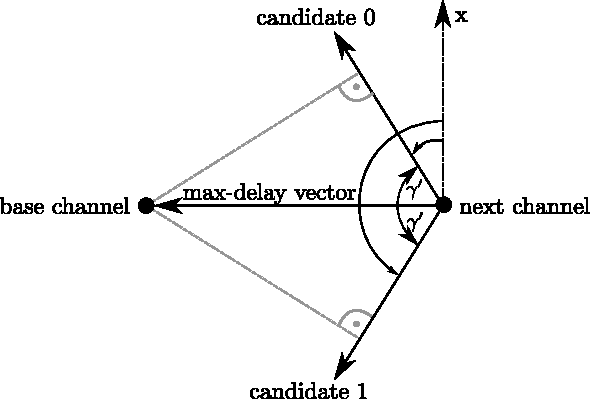
\includegraphics[width=0.6\columnwidth]{figures/tdoa_code}
	\caption{Illustration of the resulting candidates of \ac{TDOA} implementation.}
	\label{fig:03_tdoaCode}
\end{figure}

As there exists the exceptional case that the sidewise and forward delays are both small
as considered in \cref{sec:02_distance}, the invalidity of
\lstinline!small_y_shift && small_x_shift! as notated in \cref{lst:03_distance} must
be confirmed.
If so, not only the direction but also an approximate distance can be determined
as depicted in \cref{sec:03_distance}.
Otherwise, the direction with the smallest difference between the
candidates of each channel is submitted as final result.

A final result of the sound source direction relative to one robot must be defined
a the eight candidates of the four delays.
Therefore, the sum of the difference for each combination of the candidates
is taken as decisive criterion to find a final direction angle $\gamma$ in robot coordinates.
During research, different factors like signal strength were tested to include
more properties of the signal. They will be topic in \ref{sec:04_direction}.